\chapter{Use Case} 

This chapter teaches user how to use Teakwood. Teakwood is designed for scientific researcher's daily use, so a simple submitting logic is very important. Since computing tools varies, the way of submit a jobs may different, so Teakwood create a maximized general flow, which makes it suiting most of the computing tools. \\

\section{Job Submission Flow}
Fisrt let's take a look at the classical job submission flow in Teakwood.
\begin{figure}[h]
\centering
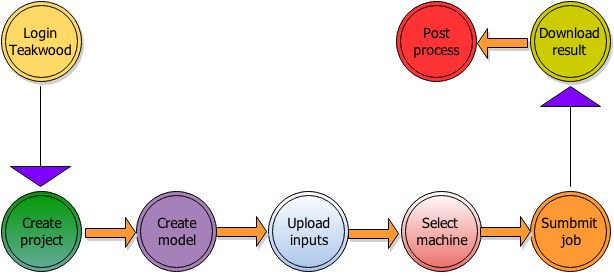
\includegraphics[scale=0.6]{./submission}
\caption{Job Submission Flow}
\label{fig:label} % insert suitable label, this is used to refer to a fig from within the text as shown above
\end{figure}

Let's go to the details of each circle in the upper figure:\\

$\bullet$ \textbf{Login}: Only logged user can use the working console, visitors only can see the information page.\\
$\bullet$ \textbf{Project}: A project relates to a big problem resolving. A project may use a lot of computing tools(packages), a lot of models, a lot of machine in order to solve this big problem.\\
$\bullet$ \textbf{Model}:A configuration package guides the computing tool how to use inputs and machines.\\
$\bullet$ \textbf{Inputs}: Data that will be used during the computing.\\
$\bullet$ \textbf{Machine}: Where your job runs.\\
$\bullet$ \textbf{Job}: a single running on a single machine.\\
$\bullet$ \textbf{Result}: Final output of the job running.\\
$\bullet$ \textbf{Post-process}: refine the output data, visualize the data, validate the data, etc.\\
\section{Job Monitoring}
In order to let user have a better view of their job status, Teakwood provides a five- stage monitoring. \\

$\bullet$ \textbf{Uploading}: means your job is sending to the remove machine.\\
$\bullet$ \textbf{Queued}: means your job is accepted and placed in the to-run list.\\
$\bullet$ \textbf{running}: means your job is running status.\\
$\bullet$ \textbf {Finished}: means you finished your job or your hour is used over.\\
$\bullet$ \textbf{Data Ready}: means your data is synchronized to file server and ready for download.\\
\section{Download output}
Directly go to the report page and download your output result. you've done your job.